\subsubsection{Kokkos - Euler Equation}
\graphicspath{ {./images/} }

开始挖坑,主要是最近比较闲(划掉),开始准备准备面试啥的,把之前的分析和代数都翻出来看看,
以及材力,弹性力学,但流体主要是看个乐子,买了本DG的书到现在还没翻过,本着买了不看是
浪费的原则,打算认证的学习一下,为了能够不是盲目的两眼抹黑。

使用Kokkos和Deal.II两个库进行
学习,github上有这两个库的Euler气体方程的计算案例,Kokkos使用的是FVM进行求解(主要FEM的
自由度处理比较抽象,还有RT单元的基函数),Deal.II使用的是DG进行计算(除了电磁的单元)
没见过用到5阶单元的,自由度数量非常多,下面的图是9.2M自由度跑出来的结果,在3马赫下的圆柱
扰流,据作者自己说服务器跑了一天才搞定,具体的两个项目可以点击查看
\href{https://github.com/pkestene/euler2d_kokkos}{Kokkos FVM Euler}以及
\href{https://github.com/conservation-laws/ryujin}{Deal.II DG Euler/Compressible NV}

\begin{figure}[htbp]
    \centering
    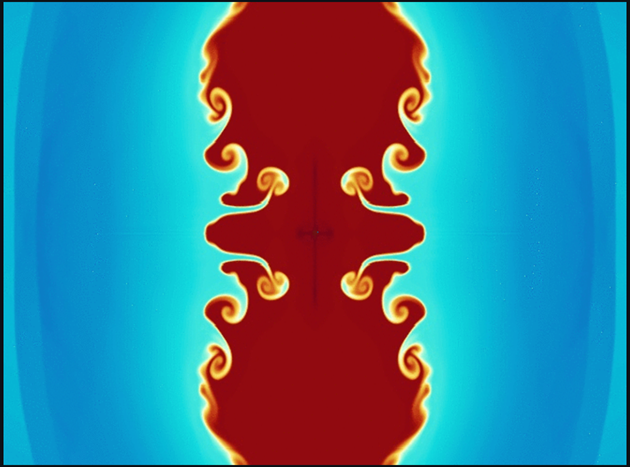
\includegraphics{FVM.png}
    \caption{FVM-Euler方程计算结果}
    \label{fig:FVM}
    \end{figure}


\begin{figure}[t]
    \centering
    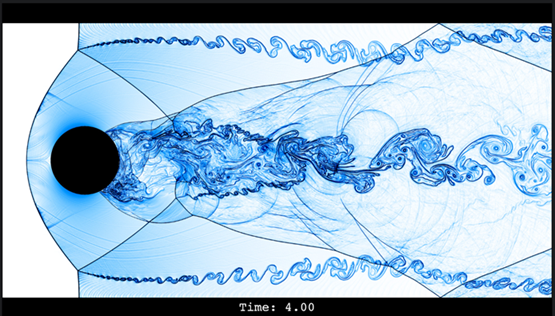
\includegraphics{DG.png}
    \caption{DG-Euler方程计算结果}
    \label{fig:DG}
    \end{figure}

Kokkos具体的技术其实主要是利用这个架构,真正意义上的预处理,GMG,AMG,之类的东西是没有的,
基本上就是一个SOR,BlockJacobi作为预处理,简单看了一下,规整网格,写了一个读取配置的,
输出vti的,好处是可以开启SIMD加速,以及可以在GPU上跑,但其实我觉得没有好的预处理感觉
规模稍微大点就是一眼寄。 

DG比较抽象,涉及到分块矩阵的预处理,正交补,以及这个方程本身就是个非线性方程,一般牛顿-
辛普森方程的雅可比矩阵还得处理一下,时变问题的CN离散方法,顺便一提这位直接不想写非线性
的雅可比,使用是自动微分,主打一个看不懂,以及网格自适应(只能说还好不是p自适应)

顺便一说,这东西我是纯粹看个乐子,主打一手开心,顺便比较一下FVM和DG的差别,目前按照我的理解
,FVM是0阶的DG,但我印象里面DG对于第一类边界条件是添加在弱形式里面,或者加上惩罚,不知道
FVM的边界是什么情况。为了能够看明白这个东西,将会从比较简单的运输方程到斯托克斯到ins,最后到
Euler,至于什么迎风修正,SUPG之类后面再看看。

将从DG开始,看看这个运输方程是怎么解的,到时候会对比一下连续单元和DG单元的计算结果,看看表面
的跳动怎么样。至于说流体力学是什么,我反正不知道,我只会方程离散到弱形式,为什么这样,以及一些结论可谓
一窍不通,单纯的从方程到离散求解的过程。关于自动微分之前解非线性的时候用过一两回,我只能说用过的
都说好,求什么变分导数,感觉不如残差线性化,尤其对于两相流这样的几个方程套在一起,再掺和一个
水平集描述,可谓是群贤毕至,满汉全席,为了身心健康着想,还是自动微分实在,放弃智力,拥抱现代
c++模板。

最后看看能不能衔接上occt参数化建模优化一下经典的翅膀形状,又是最不想动脑的一集,直接自动微分,
时变问题直接离散伴随,优化LP,顺便看看能不能调一下Tpetra让代码在GPU上跑跑。